\chapter{Grundlagen}

Dieses Kapitel stellt die Grundlagen der Arbeit dar. Diese bestehen aus den verschiedenen Service-Modellen des Cloud Computings, welche definiert und voneinander abgegrenzt werden. Darauf folgt ein Abschnitt, der die nötigen Tools der Anwendungen sowie weitere dieser Art vorstellt.

\section{Service-Modelle}

Einer der Vorreiter des Cloud Computing ist John McCarthy, der in einer Rede am Massachusetts Institute of Technology (MIT) 1961 den Begriff des Utility Computings prägte. In dieser Rede ging er davon aus, dass in der Zukunft Rechenleistung ebenso wie das Telefonsystem als öffentliche Versorgung organisiert sind. Vergleichbar soll diese Versorgung dann mit Wasser, Strom und Gas sein. Entsprechend haben sich bis heute einige große Cloud-Anbieter wie \ac{AWS}, Google Cloud Platform oder Microsoft Azure entwickelt. Deren Geschäftsmodell begann damit, dass sie ihre überschüssige Rechenleistung als öffentlichen Dienst angeboten haben. Dies wird aber mehr und mehr zum Kerngeschäft dieser Unternehmen. \autocite{buyya2013mastering}

Allgemein lässt sich die Cloud in verschiedene Service-Modelle wie \ac{IaaS}, \ac{PaaS}, \ac{FaaS}, \ac{BaaS} oder \ac{SaaS} unterteilen. Die Definition, Abgrenzung und Einordnung dieser Modelle und Begriffe wird in verschiedener Literatur \autocite{jiang2020overview}\autocite{kumar2019serverless}\autocite{dahunsi2021commercial} behandelt. Zusätzlich ist noch zu erwähnen, dass schlussendlich alles als Dienst angeboten werden kann. So hat sich \ac{XaaS} etabliert. Weitere Beispiele für die solche Cloud-Dienste angeboten werden, sind AI as a Service, API as a Service, Analytics as a Service oder Knowledge as a Service.

\subsection{\acl{IaaS}}

Bei \acf{IaaS} stellt der Anbieter dem Kunden Infrastrukturelemente für eine Software bereit. Beispiele für solche Elemente sind virtuelle Maschinen, Server, Speicherplätze und Netzwerke. Bei \ac{AWS} gibt es für die genannten Beispiele die \ac{EC2}. In der Google Cloud Platform ist es die Compute Engine. In der Regel zahlt der Kunde nur für das, was er in einem bestimmten Zeitabschnitt tatsächlich genutzt hat.

Der Vorteil liegt darin, dass auf Grund der Vertragsstruktur jederzeit neue Elemente hinuzugebucht oder gekündigt werden können. Das macht \acl{IaaS} flexibler und skalierbarer gegenüber dem herkömmlichen Ansatz, Server für eine bestimmte Vertragslaufzeit zu mieten oder gar vollständig zu erwerben. Auch soll ein Anreiz sein, dass dies gegenüber dem herkömmlichen Ansatz kostengünstiger ist.

Nachteilig ist allerdings, dass die Server in einem externen Rechenzentrum liegen und somit die Sicherheit nicht in der eigenen Hand liegt, was eine gängige Herausforderung beim Cloud Computing darstellt. So wie bei allen weiteren Service-Modellen benötigt der Kunde eine stetige Internetverbindung zum Server, selbst wenn es sich nur um eine firmeninterne Anwendung handelt.

\subsection{\acl{PaaS}}

\acf{PaaS} baut auf \acl{IaaS} auf und bietet zusätzlich eine Entwicklungsplattform mit Tools zum Entwickeln als Dienst an. Beispiele für \ac{PaaS} sind \ac{AWS} Elastic Beanstalk, Google App Engine und Heroku.

Die Vor- und Nachteile von \acl{IaaS} treffen hier auch zu. Zusätzlich ist ein Vorteil, dass der Kunde sich nicht mehr selbst um die Hard- und Software kümmern muss, sondern sich lediglich auf die Entwicklung von Software-Produkten fokussieren kann. Der Anbieter selbst wickelt die Wartung und Pflege ab. Ein Nachteil ist, dass Entwickler keinen Einfluss auf die Umgebung selbst nehmen können, falls sie diese im Zweifelsfall verändern müssen.

\subsection{\acl{FaaS}}

Die Domänenlogik einer Anwendung kann mittels \acf{FaaS} abgebildet werden. Es handelt sich um Funktionen, die mit Parametern über Trigger aufgerufen werden können. Solch eine Funktion liegt nicht auf eigenen Servern, sondern beim jeweiligen Anbieter. Die Abgrenzung zu \ac{PaaS} ist, dass es sich hierbei nur um Funktionen handelt, während es sich bei \ac{PaaS} um eine ganze Anwendung handelt. Somit entsteht bei \ac{FaaS} die Anwendung dadurch, dass beispielsweise ein API-Gateway die Funktion aufruft. Beispiele für \ac{FaaS} sind \ac{AWS} Lambda, Google Cloud Functions, Azure Functions oder IBM OpenWhisk.

Ein Vorteil von \ac{FaaS} ist die Skalierbarkeit, die vom Anbieter selbst verwaltet wird. Außerdem ist \ac{FaaS} plattformunabhängig, so dass in jeder angebotenen Programmiersprache entwickelt werden kann. Dadurch, dass nur das bezahlt wird, was auch genutzt wird, ist \ac{FaaS} in der Regel kostengünstiger als dauerhaft einen Server laufen zu lassen. Des Weiteren bieten die meisten Anbieter auch schon direkt Anbindungen zum Logging und Monitoring ein, was die Überwachung der Funktionen vereinfacht.

Ein Nachteil von \ac{FaaS} sind beispielsweise die Startzeit von Funktionen. Je größer der Speicherplatz einer Funktion ist, desto länger dauert die Startzeit von Funktionen. Möchte der Entwickler keine Aufwärmzeit, muss für Provisioned Concurrency bezahlt werden. Ein weiterer Nachteil ist, dass Funktionen eine maximale Ausführungsdauer haben, welche von Cloud-Anbieter variiert. Für größere Workloads muss dann eine Alternative gefunden werden.

\subsection{\acl{BaaS}}

\acf{BaaS}, auch \ac{MBaaS} genannt, wenn es speziell um mobile Applikationen geht, zielt darauf ab, dass Entwickler im Backend auf bereits bestehende Schnittstellen zugreifen können, um gängige Herausforderungen mit möglichst wenig Quellcode lösen zu können. Die folgende Auflistung gibt eine erste Übersicht über die oftmals schon vorhandenen Schnittstellen:
\begin{itemize}
  \item Authentifizierung- und Autorisierung
  \item Hosting
  \item Datenbank-Management
  \item Push Notifications
  \item Storage
  \item Analytics
  \item Geo-Dienste
  \item Maschinelles Lernen
\end{itemize}

Der Fokus wandert damit vom Backend hin zum Frontend, welches die Schnittstellen aufruft. Dennoch gibt es auch im Backend Quellcode, der geschrieben werden muss. Dies erfolgt wieder über Funktionen durch \ac{FaaS}. \ac{AWS} Amplify und Firebase lassen sich in die Kategorie der \ac{BaaS} eingliedern. Wird \ac{BaaS} mit \ac{FaaS} kombiniert, spricht man nach Mike Roberts auch von Serverless \autocite{brandon2017serverless}.

Die Vor- und Nachteile sind nahezu deckungsgleich mit denen von \ac{FaaS}. Es lässt sich noch hinzufügen, dass der Vendor lock-in bei \ac{BaaS} sich nochmal vergrößert, da viele verschiedene Dienste eines einzelnen Anbieters genutzt werden. Außerdem kann das Debugging und Monitoring auf Grund verschiedener Dienste komplexer als in üblichen Anwendungen werden.

\subsection{\acl{SaaS}}

\ac{SaaS} ist die gesamte Applikation als Dienst für den Endnutzer. Meistens ist eine Software dieser Art über ein oftmals monatliches Abonnement zu erhalten. Beispiels für Proukte dieser Art sind Slack, Microsoft 365, Salesforce oder Atlassian Jira.

Der Vorteil bei \ac{SaaS} ist, dass nicht die gesamte Software gekauft und bereitgestellt werden muss. Außerdem liefert der Hersteller regelmäßige Updates. Der Kunde muss sich also in der Regel nur noch um die Konfiguration der Anwendung selbst kümmern, während der Rest vollständig übernommen wird. Nachteilig ist damit allerdings auch, dass der Nutzer kaum Kontrolle über das Produkt hat. Des Weiteren liegen die Daten auch hier wieder auf einem externen Rechenzentrum, was auf Grund von Datensicherheit und der Datenschutz-Grundverordnung eine Hürde darstellt.

\subsection{Abgrenzung der Begriffe}

\begin{table}[h]
  \caption{Vergleich von Service-Modellen \autocite{jiang2020overview}}
  \label{Kap2:ServiceModelleVergleich}
  \renewcommand{\arraystretch}{1.2}
  \centering
  \sffamily
  \begin{footnotesize}
    \begin{tabular}{l l l l l}
    \toprule
    & \textbf{\ac{IaaS}} & \textbf{\ac{PaaS}} & \textbf{\ac{FaaS}} & \textbf{\ac{SaaS}}\\
    \midrule
    \textit{Entwicklungseffizienz} & Gering	&	Mittel	& Hoch & Hoch\\
    \textit{Skalierbarkeit} & Gering	&	Mittel & Hoch & Hoch\\
    \textit{Wartung} &	Gering	&	Hoch & Hoch & Hoch\\
    \textit{Kosten}	&	Hoch		&	Hoch & Gering & Hoch\\
    \textit{Anwender}	&	Administrator		&	Entwickler & Entwickler & Anwender\\
    \bottomrule
    \end{tabular}
  \end{footnotesize}
  \rmfamily
\end{table}

\autoref{Kap2:ServiceModelleVergleich} vergleicht \ac{IaaS}, \ac{PaaS}, \ac{FaaS}, damit implizit auch \ac{BaaS}, und \ac{SaaS} anhand den Kriterien Entwicklungseffizienz, Skalierbarkeit, Wartung, Kosten und den Anwendern.

Von links nach rechts nimmt dabei der Fokus auf die Business-Logik zu. Während bei \ac{IaaS} nur Infrastrukturelemente bereitgestellt werden, wird bei \ac{SaaS} die ganze Anwendung bereitgestellt. Dem entsprechend nimmt auch die Abstraktion von links nach rechts zu. Folglich nimmt die Flexibilität ab, da der Anwender bei \ac{SaaS} höchstens noch die Anwendung konfigurieren kann. Zwischen \ac{PaaS} und \ac{SaaS} hat \ac{FaaS} den Vorteil, dass dieser Dienst noch für Entwickler gedacht ist und damit flexibel genug ist, um Anwendungen aufzubauen. Dieser Vorteil trifft entsprechend auch auf \ac{BaaS} zu. \ac{FaaS} und \ac{BaaS} stellen alle nötigen Ressourcen exklusive des Anwendungslogik zur Verfügung.

\begin{figure}[h]
  \centering
  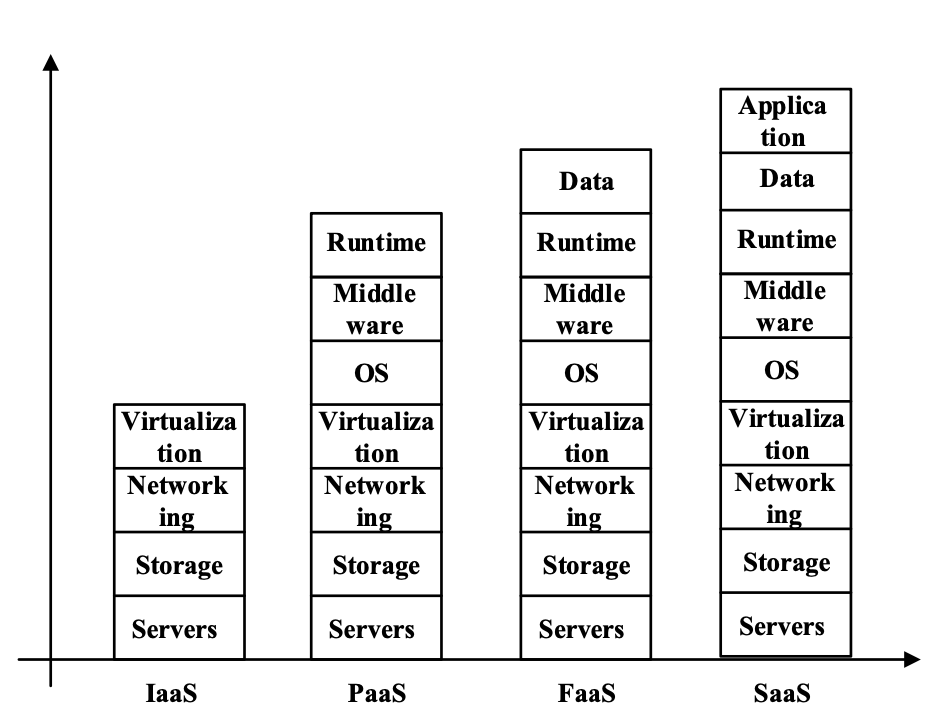
\includegraphics[width=0.75\columnwidth]{2_grundlagen/vergleich-service-modelle.png}
  \caption{Vergleich der Elemente von Service-Modellen \autocite{jiang2020overview}}
  \label{Kap2:VergleichServiceModelleElemente}
\end{figure}

\autoref{Kap2:VergleichServiceModelleElemente} vergleicht die Service-Modelle ebenfalls uns zeigt auf, welche Elemente von welchem Modell geliefert werden. Dabei ist auffällig, dass von links nach rechts mehr Elemente bereitgestellt werden. Für die Neuentwicklung von Anwendungen bedeutet das, dass \ac{FaaS} und \ac{BaaS} geeignet sind, da nur die Anwendungslogik geschrieben werden muss und die restlichen Elemente vom Anbieter selbst kommen.

\section{Anbieter von \acl{BaaS}}

\subsection{AWS Amplify}

\subsubsection{Placeholder 1}
\subsubsection{Placeholder 2}

\autocite{dahunsi2021commercial}
\autocite{amplifyDocs}
\autocite{lysakov2021security}
\autocite{mathew2014overview}
\autocite{beach2014aws}

  - Amplify
  - Amplify CLI
  - Custom Plugins
  - Wie sieht die Infrastrutkur aus, wie der code, wie das frontend?
  - CloudFormation
  - AppSync
  - Lambda
  - S3
  - Cognito
  - MediaConvert
  - Amazon EventBridge
  - DynamoDB
  - CloudFront (weil kurz erwähnt)

\subsection{Firebase}

\subsubsection{Placeholder 1}
\subsubsection{Placeholder 2}

\autocite{moroney2017definitive}
\autocite{firebaseDocs}
\autocite{tanna2018serverless}

- Weitere BaaS tools

Allgemeines:
  - Anzahl der Nutzer
  - Zufriedenheit / Akzeptanz
  - Zeit im Markt
  - Sonstige Fakten
  - GitHub Stars

\subsection{Weitere Anbieter}

todo